% Author : Ali Snedden
% Date   : 10-feb-2022
% License: MIT (for my content), images licensed appropriately
% Purpose: 
%   This is my nerd hour presentation for the Batelle Center for Mathematical Medicine
% 







\documentclass{beamer}
\usetheme{Copenhagen}
%\usecolortheme{seahorse}
% See http://www.hartwork.org/beamer-theme-matrix/ for more themes and colors

\usepackage{times}  % fonts are up to you
\usepackage{graphics}
\usepackage{amsmath}
\usepackage{media9}
\usepackage{hyperref}

\usepackage{tikz}
\usetikzlibrary{fit}

%Bibliography stuff
%\usepackage[style=authoryear]{biblatex}
\bibliography{/Users/ali/Library/texmf/bibtex/bib/references}
%\bibliographystyle{apj}

\setbeamertemplate{bibliography item}[text]
%\usepackage[backend=bibtex, style=authoryear]{biblatex}
%\addbibresource{/Users/ali/Library/texmf/bibtex/bib/references.bib}
\newcommand{\customcite}[1]{\citeauthor{#1}, \citeyear{#1}}
% https://tex.stackexchange.com/a/61016/84495
\newcommand{\chref}[3][blue]{\href{#2}{\color{#1}{#3}}}%


\newcommand\smallFont{\fontsize{8}{7.2}\selectfont}   %Change font size.
\newcommand\mCite[1]{[\cite{#1}, \citetitle{#1}]}  %Prints name and title
\newcommand\FrameText[1]{
\begin{textblock*}{\paperwidth}(0pt,\textheight)
    \vspace{1.0cm}
    \raggedleft \smallFont #1
\end{textblock*}}

%Get rid of ugly copenhagen default symbol for enumerate
\setbeamertemplate{enumerate items}[default]   

%Increase default separation size between items in itemize and enumerate 
\tikzset{type1/.style={rectangle, rounded corners, minimum width=3cm, minimum height=0.1cm,text centered, draw=black, fill=blue!10, text width=2cm},
        type2/.style={rectangle, rounded corners, minimum width=3cm, minimum height=0.1cm, text centered, draw=black, fill=blue!10, text width=5cm},
        info/.style = {rectangle, rounded corners, minimum width=2.5cm, minimum height=0.1cm, text centered, draw=black, 
            fill=blue!30, text width=2.5cm},
        org/.style={rectangle, rounded corners, minimum width=2cm, minimum height=0.1cm, text centered, draw=black, 
            fill=blue!30, text width=3cm},
        decision/.style = {square, minimum width=1cm, minimum height=0.1cm, text centered, 
            draw=black, fill=green!30, text width=4cm},
        arrow/.style = {thick,->,>=stealth},
    }
    
    
    
   

%%%%%%%%%%%%%%% BIBLIOGRAPHY COMMANDS %%%%%%%%%%%%%%%
\newcommand{\apj}{ApJ.}
\newcommand{\apjs}{ApJS}
\newcommand{\apjl}{ApJL}
\newcommand{\pasp}{Publications of the Astronomical Society of the Pacific}
\newcommand{\pasj}{Publ. of the Astron. Soc. of Japan}
\newcommand{\prc}{Phys. Rev. C}
\newcommand{\prd}{Phys. Rev. D}
\newcommand{\nat}{Nature}
\newcommand{\mnras}{Mon. Not. R. Astron. Soc.}
\newcommand{\na}{New Astronomy}
\newcommand{\aap}{Astronomy and Astrophysics}
\newcommand{\araa}{Annu. Rev. Astron. Astrophys}
\newcommand{\aj}{Astronomical Journal}
\newcommand{\pasa}{Pub. of the Astron. Soc. of Australia}
\newcommand{\nar}{New Astronomy Reviews}


%%%%%%%%%%%%%%% OTHER COMMANDS %%%%%%%%%%%%%%%%%
\newcommand{\subitem}{\item[$-$]}

% these will be used later in the title page
\title{Is anyone out there?}
\author{Ali Snedden
}
\date{February 10, 2022}
%\subtitle{stuff}

% note: do NOT include a \maketitle line; also note that this title
% material goes BEFORE the \begin{document}

% Recurring Outline
\AtBeginSection[]  % "Beamer, do the following at the start of every section"
{
\begin{frame}<beamer> 
\frametitle{Outline} % make a frame titled "Outline"
\tableofcontents[currentsection]  % show TOC and highlight current section
\end{frame}
}

\begin{document}

% this prints title, author etc. info from above
\begin{frame}
\titlepage
\end{frame}





%%%%%%%%%%%%%%%%%%%%%%%%%%%%%%%%%%%%%%%%%%%%%%%%%%%
%%%%%%%%%%%%%% History : Pre-Modern %%%%%%%%%%%%%%%
%%%%%%%%%%%%%%%%%%%%%%%%%%%%%%%%%%%%%%%%%%%%%%%%%%%
\section{History : Pre-Modern (pre-$20^{th}$ century)}
%%% % TO DO Cite tippler here, add pictures
\begin{frame}
\frametitle{Antiquity}
\begin{picture}(320,250) 
\put(200, 150){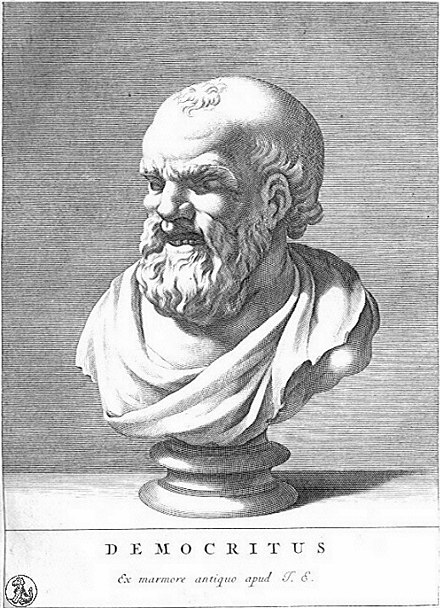
\includegraphics[height=0.75in]{images/democritus-PD.jpg}{\scriptsize{Democritus}}}
\put(200, 75){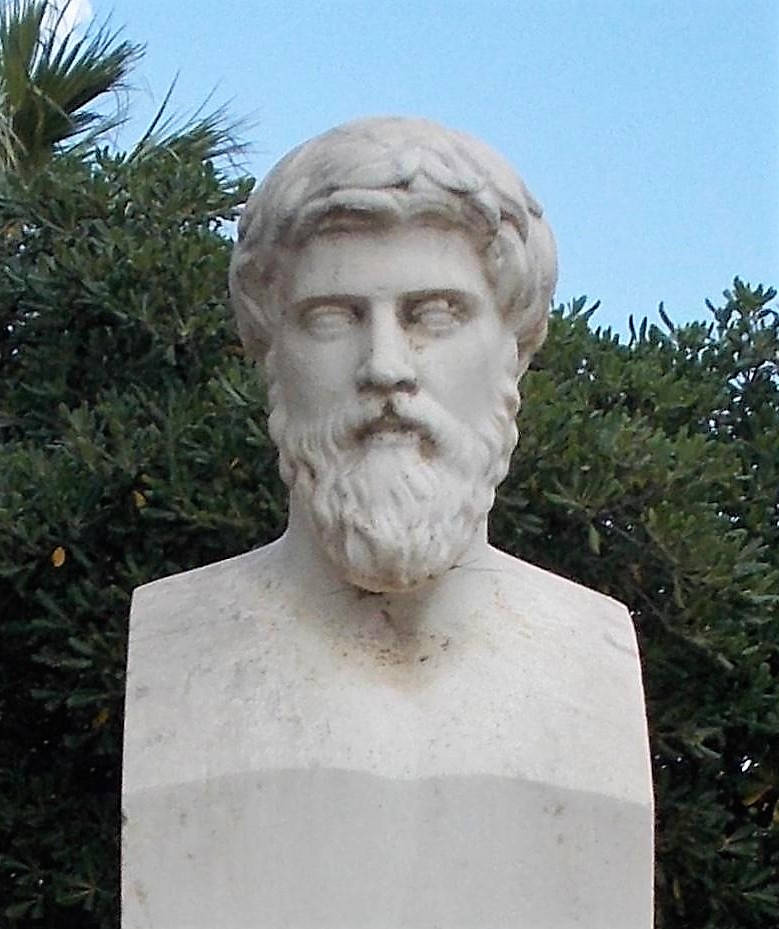
\includegraphics[height=0.75in]{images/plutarch-cc-by-sa4.jpg}{\scriptsize{Plutarch}}}
\put(-20, 250){\begin{minipage}[t]{0.6 \linewidth}
{\begin{itemize}
    \item ``Believers" in life on other planets
        \begin{enumerate}
            \item Democritus (atomic theory of the universe, geometry)
            %\put(150, 200){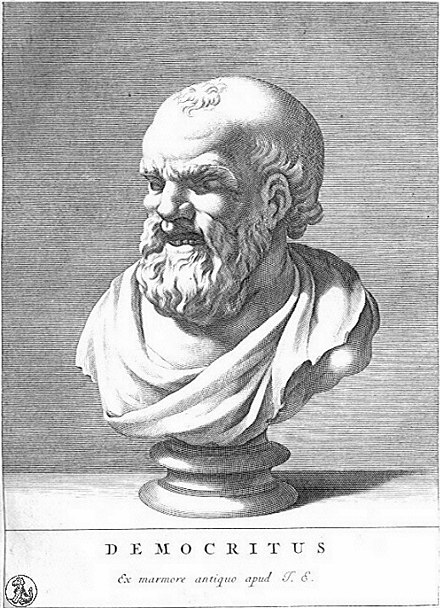
\includegraphics[height=0.75in]{images/democritus-PD.jpg}}
                %{\scriptsize{Democritus (atomic theory of universe}}
            \pause
            \item Metrodorus of Chios 
                \begin{itemize}
                    \item[--] ``It seems absurd, that in a large field only one stalk
                                should grow, and that in an infinite space only one world
                                exist."
                \end{itemize}
            \pause
            % Contmporary of Nero of fiddle fame
            \item Plutarch (historian)
        \end{enumerate}
\end{itemize}}
\end{minipage}}
\end{picture}
\end{frame}

\begin{frame}
\frametitle{Antiquity}
\begin{picture}(320,250) 
\put(200, 150){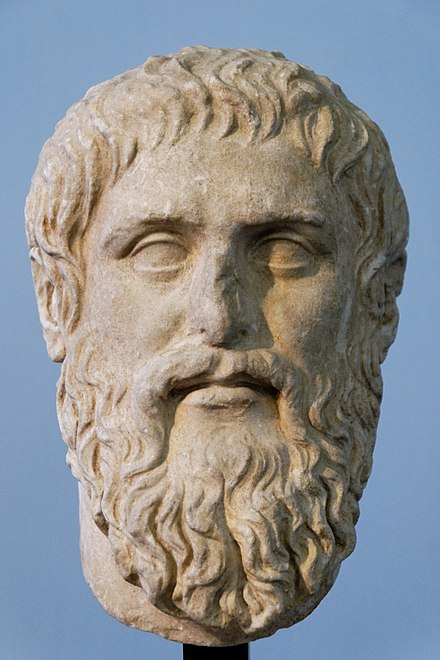
\includegraphics[height=0.75in]{images/plato-PD.jpg}{\scriptsize{Plato}}}
\put(200, 75){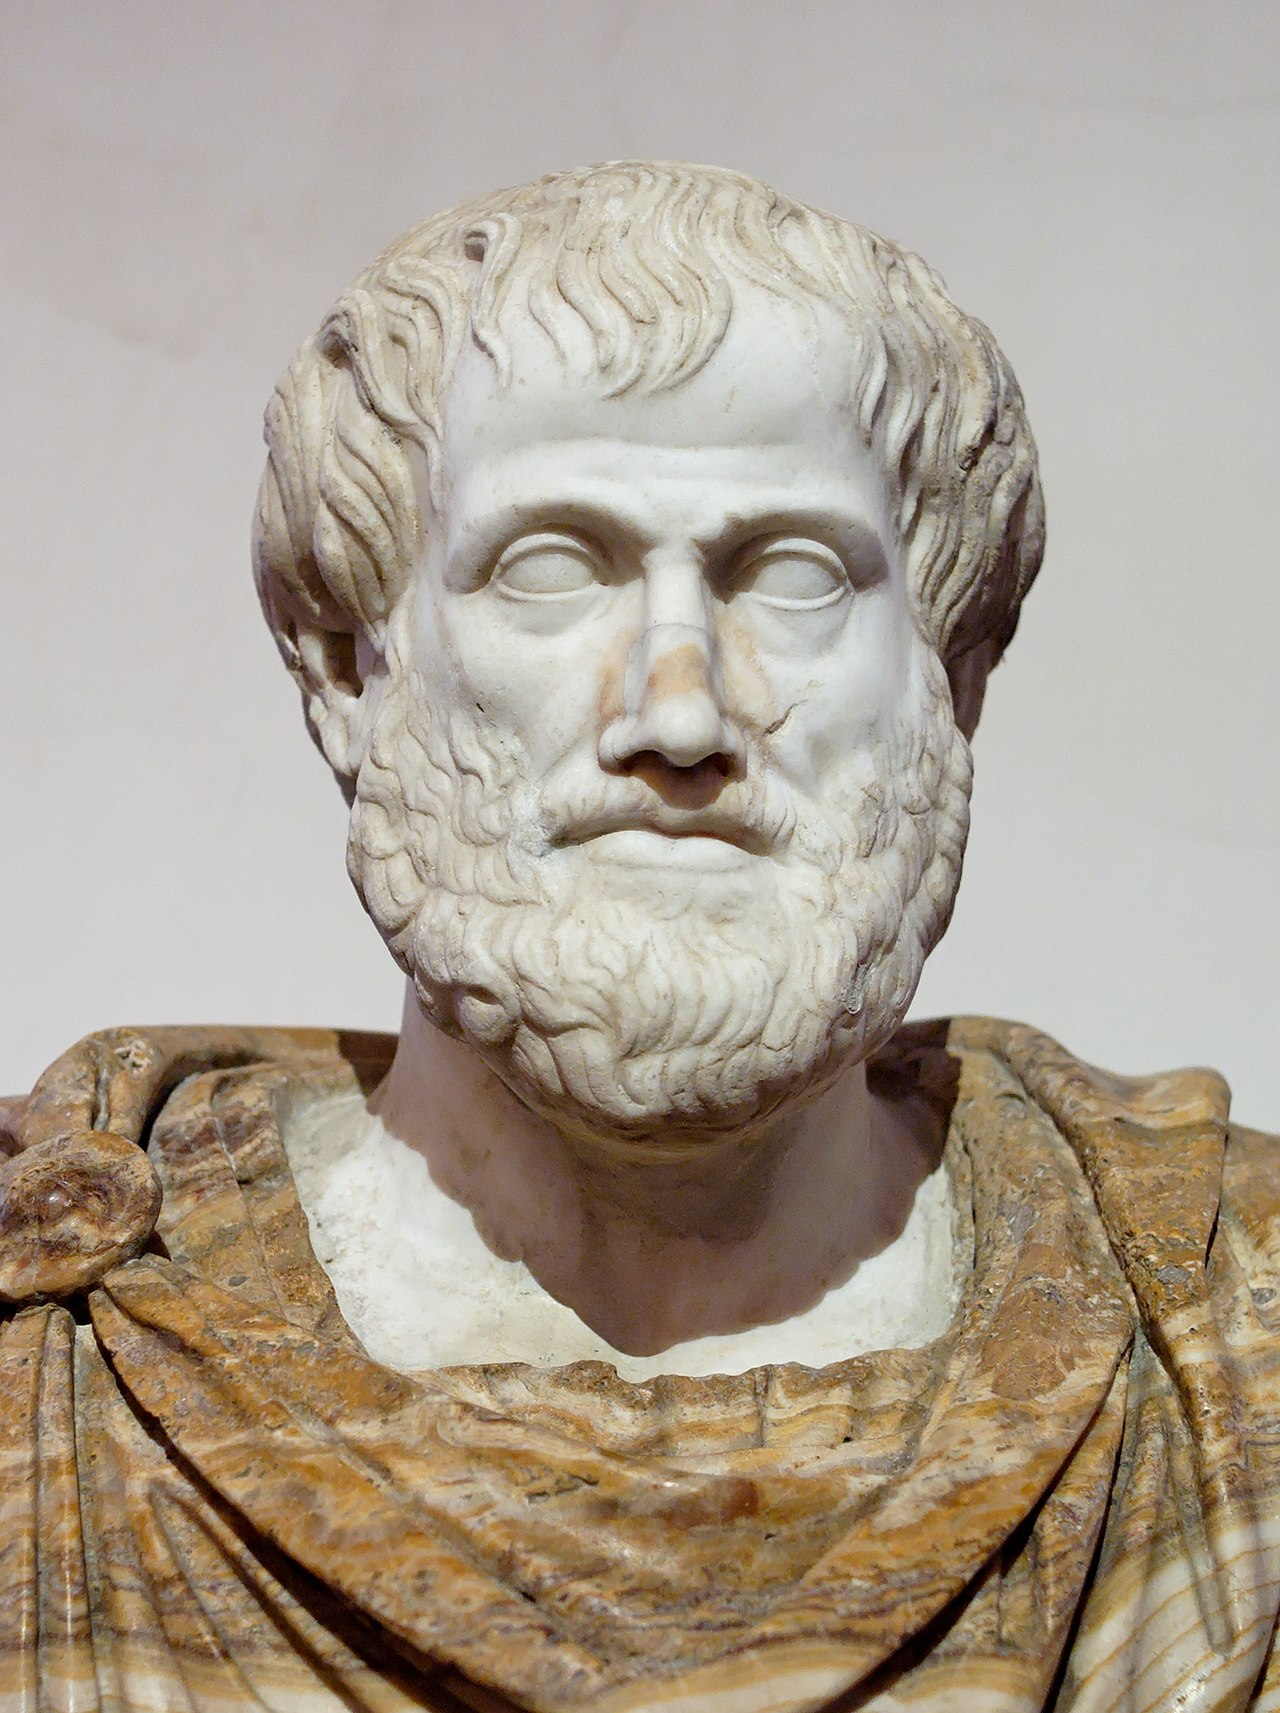
\includegraphics[height=0.75in]{images/aristotle-PD.jpg}{\scriptsize{Aristotle}}}
\put(-20, 250){\begin{minipage}[t]{0.6 \linewidth}
{\begin{itemize}
    \item ``Non-believers" in life on other planets
        \begin{enumerate}
            \item Plato (philosopher)
            \pause
            \item Aristotle (philosopher)
                \begin{itemize}
                    \item[--] Universe of Aristotle is finite, with only one inhabited planet
                \end{itemize}
        \end{enumerate}
\end{itemize}}
\end{minipage}}
\end{picture}
\end{frame}

\begin{frame}
\frametitle{Christian Era}
\begin{picture}(320,250) 
\put(200, 150){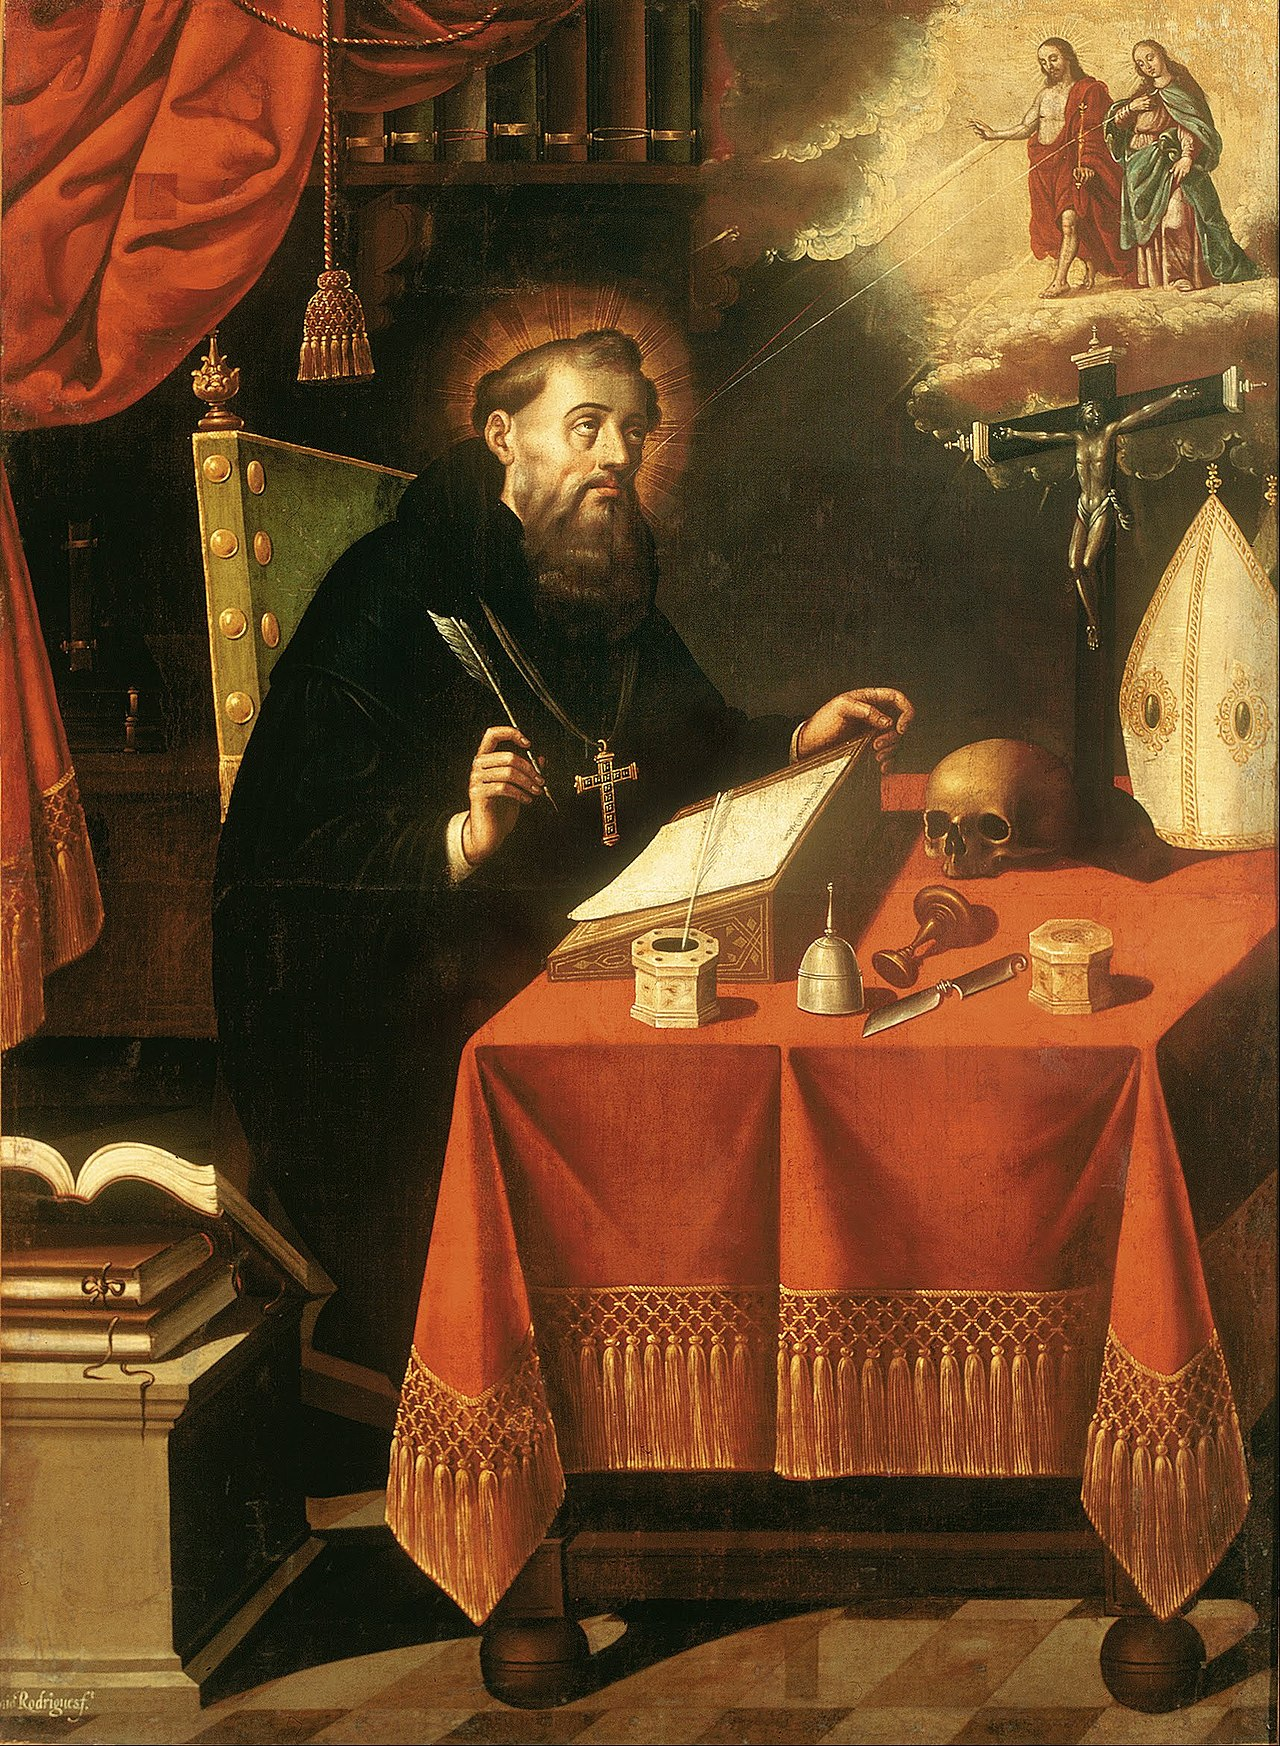
\includegraphics[height=0.75in]{images/st-augustine-PD.jpg}{\scriptsize{St. Augustine}}}
\put(250, 100){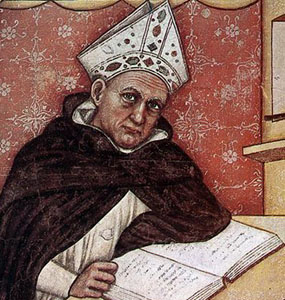
\includegraphics[height=0.75in]{images/albertus-magnus-PD.jpg}{\scriptsize{St. Albertus Magnus}}}
\put(200, 50){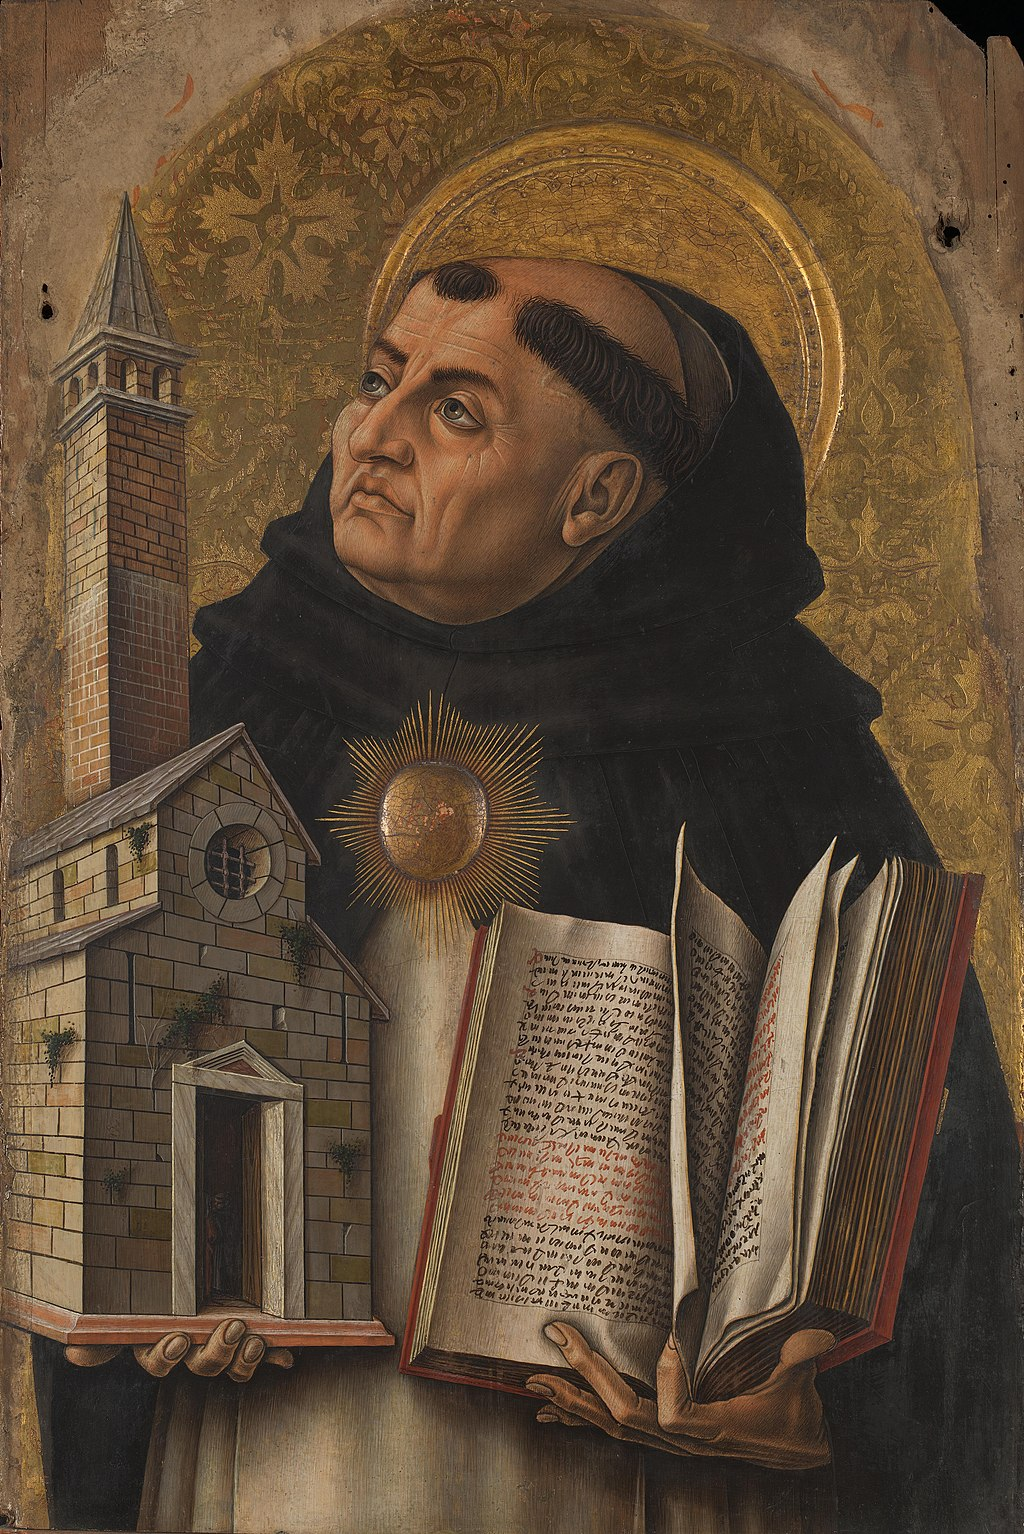
\includegraphics[height=0.75in]{images/thomas-aquinas-PD.jpg}{\scriptsize{St. Thomas Aquinas}}}
\put(-20, 250){\begin{minipage}[t]{0.7 \linewidth}
{\begin{itemize}
    \item ``Non-believers" 
        \begin{enumerate}
            \item St. Augustine (Theologian)
                \begin{itemize}
                    \item[--] If other intelligent begins similar to man existed, then they'd 
                              also require a savior, which would contradict the uniqueness of
                              Christ (I Peter 3:18)
                \end{itemize}
            % Commented on Aristotle, Discovered Arsenic
            \item St. Albertus Magnus (Friar, Philosopher, Scientist)
                \begin{itemize}
                    \item[--] "Do there exist many worlds or is there but a single world?
                              This is one of the most noble and exalted questions in the
                              study of Nature"
                \end{itemize}
            % Influential Philosopher
            \item St. Thomas Aquinas (Philosopher, Theologian)
                \begin{itemize}
                    \item[--] If God made many similar workds, they would be in vain and 
                               inconsistent with Divine Wisdom.
                \end{itemize}
        \end{enumerate}
\end{itemize}}
\end{minipage}}
\end{picture}
\end{frame}


\begin{frame}
\frametitle{Renaissance }
\begin{picture}(320,250) 
\put(200, 150){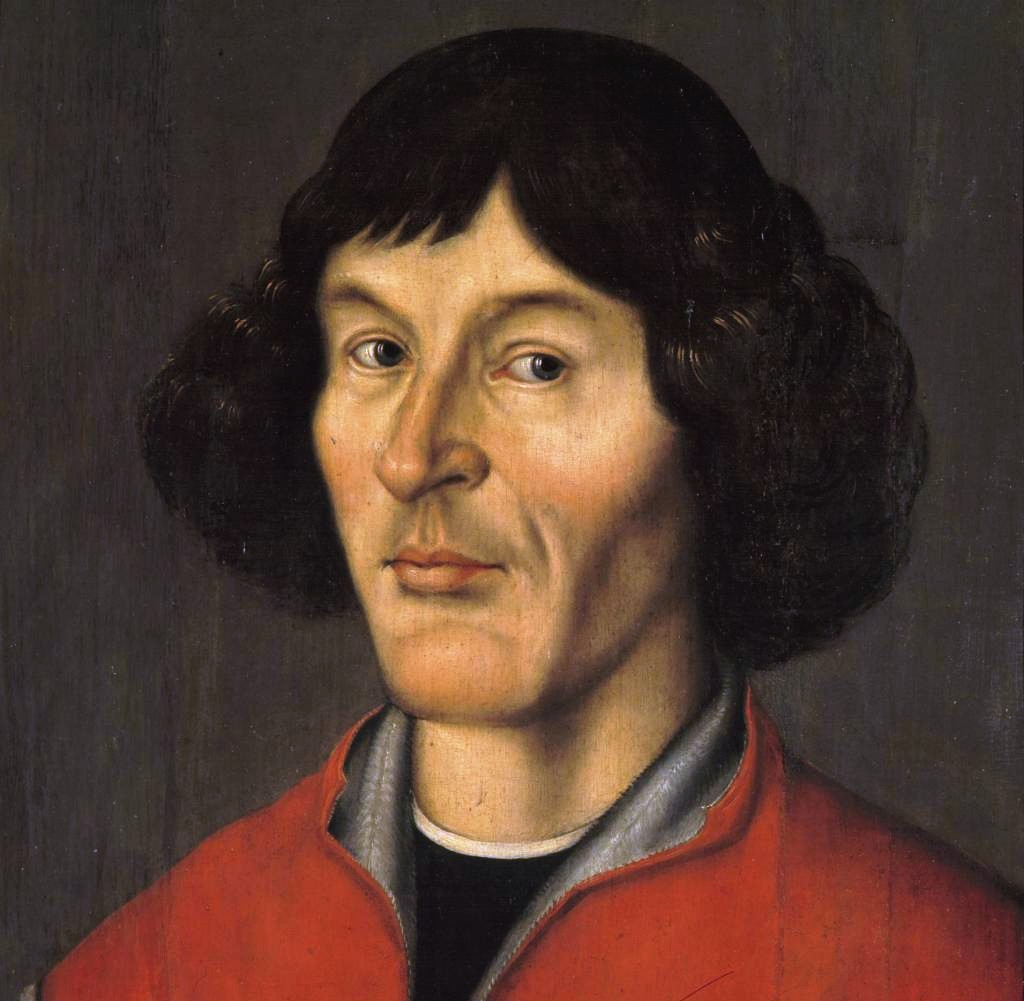
\includegraphics[height=0.75in]{images/nicolaus-copernicus-PD.jpg}{\scriptsize{Copernicus}}}
\put(250, 100){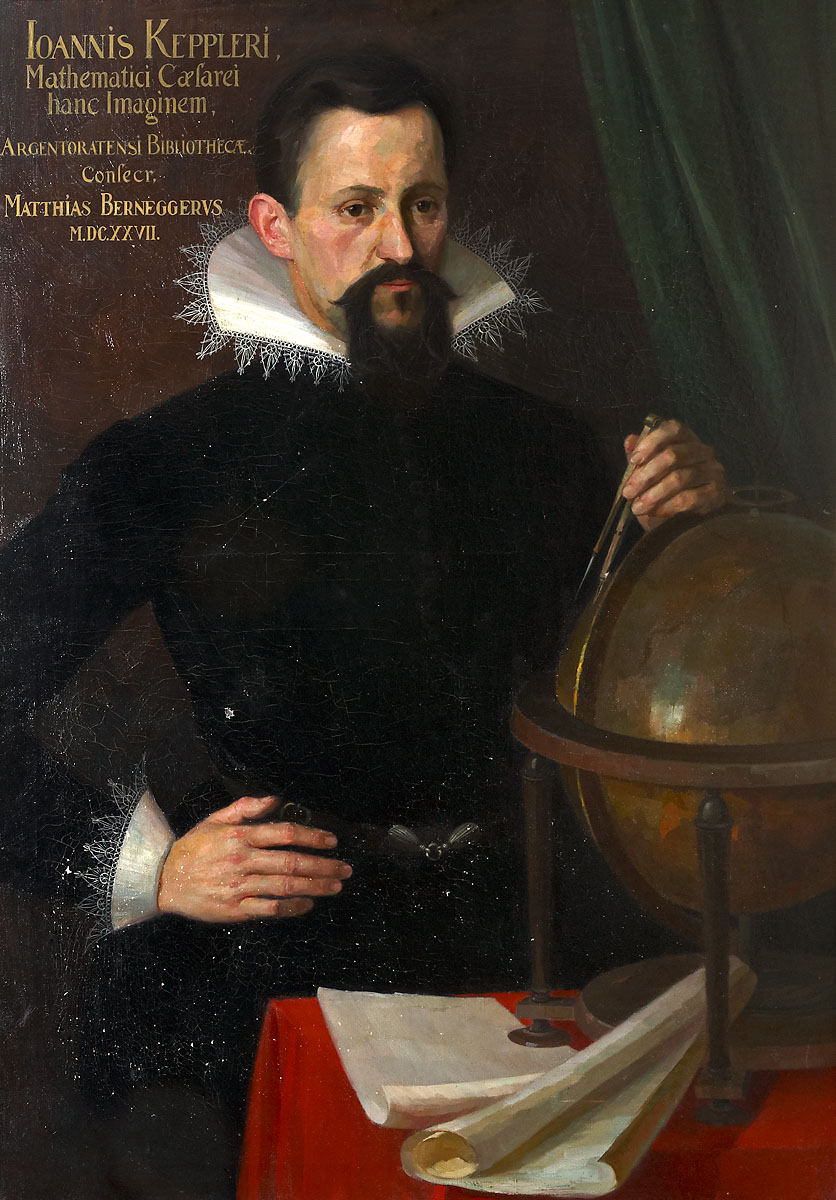
\includegraphics[height=0.75in]{images/jkepler-PD.jpg}{\scriptsize{Kepler}}}
\put(200, 50){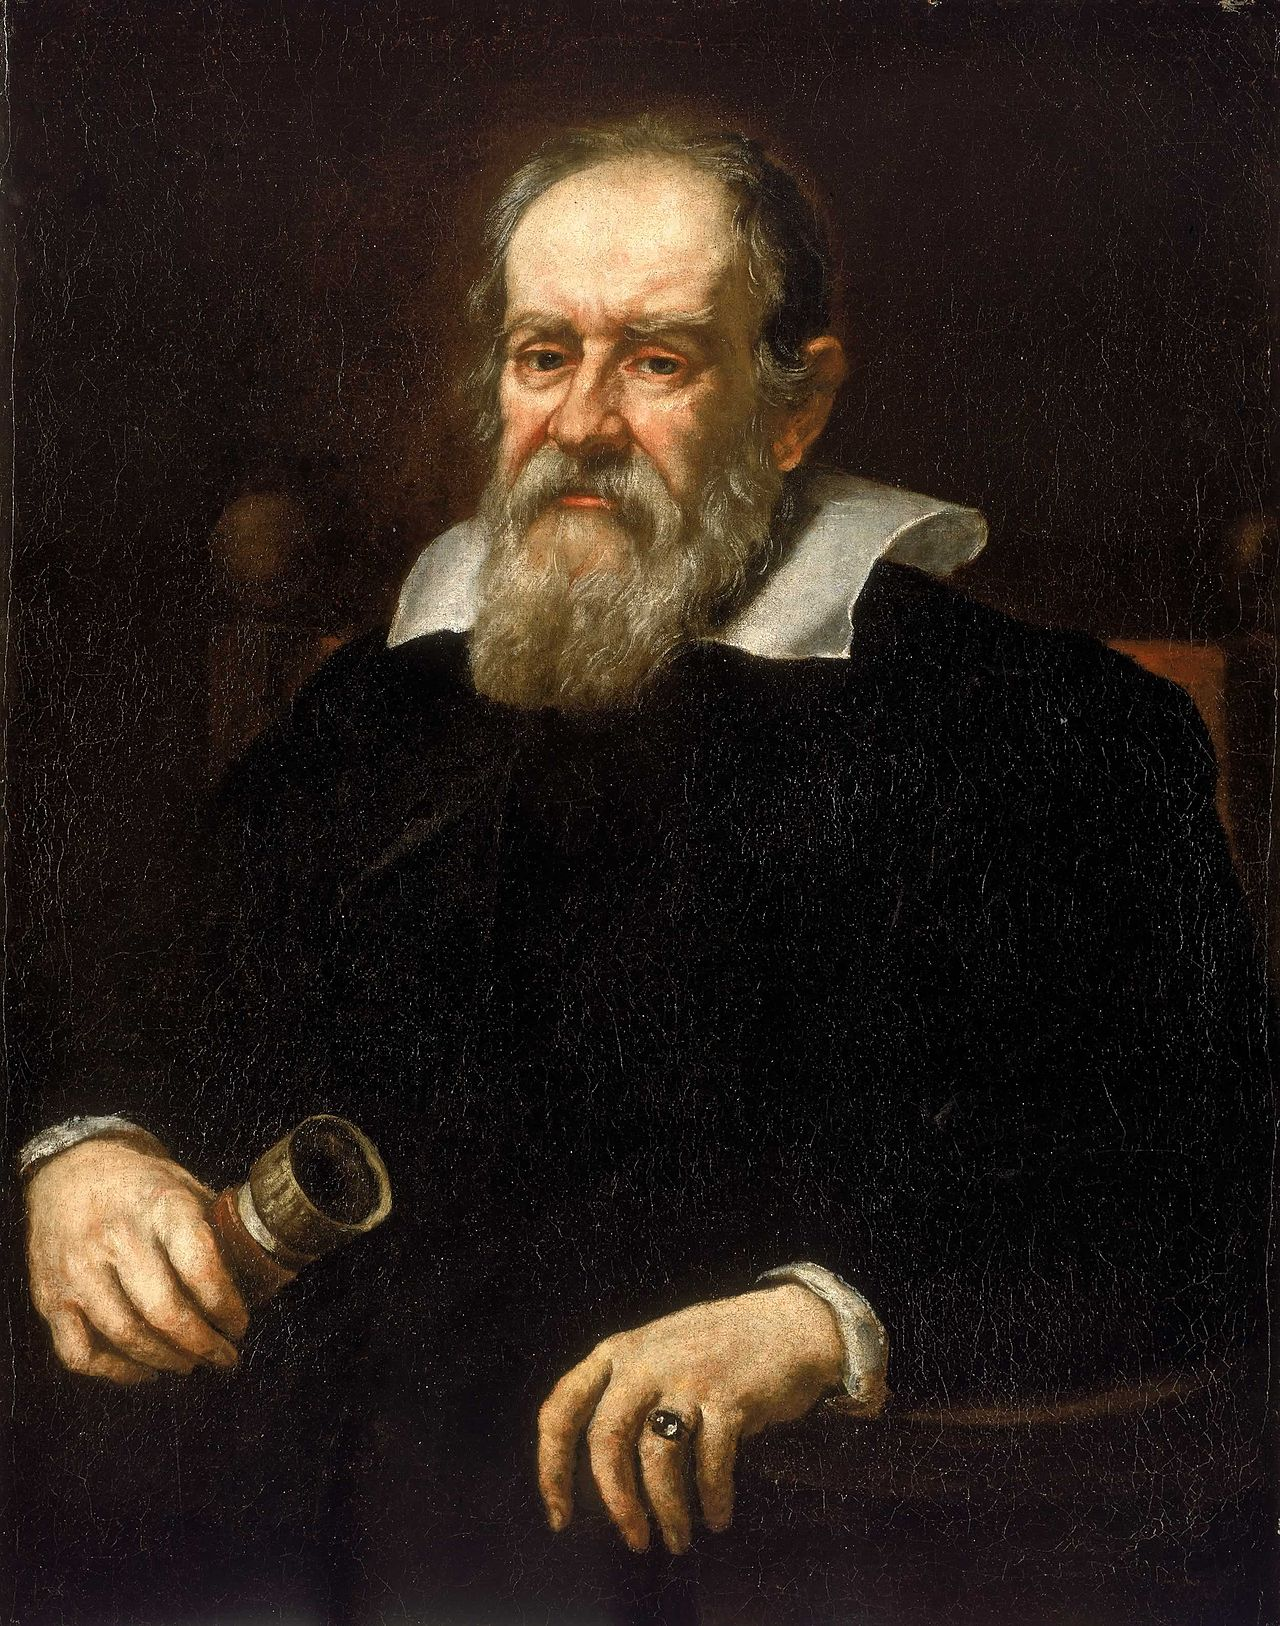
\includegraphics[height=0.75in]{images/galileo-galilei-PD.jpg}{\scriptsize{Galileo}}}
\put(-20, 250){\begin{minipage}[t]{0.7 \linewidth}
{\begin{itemize}
    \item ``Non-believers" 
        \begin{enumerate}
            % Open to intelligent life
            \item Nicolaus Copernicus 
                \begin{itemize}
                    \item[--] Believed plurality of worlds around other stars with intelligent beings
                \end{itemize}
            % Maybe life, nothing like humans
            \item Johannes Kepler
                \begin{itemize}
                    \item[--] "No moons have yet been seen revolving around [the stars].
                               Hence this will remain an open question until this
                               phenomenon too is detected"
                \end{itemize}
            % Non-believer
            \item Galileo Galilei (telescope, Jupiter's moons)
                \begin{itemize}
                    \item[--] "... false and damnable the view of those who would put
                               inhabitants on Jupiter, Venus, Saturn and the Moon, meaning
                               by 'inhabitants' animals like ours and min in particular"
                            
                \end{itemize}
        \end{enumerate}
\end{itemize}}
\end{minipage}}
\end{picture}
\end{frame}


\begin{frame}
\frametitle{Enlightenment}
\end{frame}


\begin{frame}
\frametitle{Modern Era}
\end{frame}

%%%  
%%%  
%%%  %\section{Methods}
%%%  %\begin{frame}
%%%  %\frametitle{Antiquity}
%%%  %\begin{picture}(320,250) 
%%%  %    \put(-10, 145){\includegraphics[height=1.25in]{/Users/asnedden/Documents/Professional/Talks/Nerd_hour_01_22_16/images/armenian_cave.eps}}
%%%  %    \put(25, 240){\begin{minipage}[t]{0.3 \linewidth}
%%%  %    {\scriptsize{Armenian Cave 4000BC}}
%%%  %    \end{minipage}}
%%%  %\end{frame}
%%%  
%%%  %\section{Experiments}
%%%  %
%%%  %\section{Signatures of Life}
%%%  %
%%%  %\section{Why earth isn't so special}
%%%  %
%%%  %\section{Intelligent Life}
%%%  %
%%%  % Unsolved mysteries, x-files
%%%  % Drake eqn
%%%  % Fermi paradox
%%%  % Compute energy required to travel to alpha centari.
%%%  % Government interest, 
%%%  % Omumguma
%%%  
\begin{frame}
\frametitle{Modern Era}
"There can be little doubt that civilizations more advanced than the earth's
 exist elsewhere in the universe. The probabilities involved in locating one of them
 call for a substantial effort." - Carl Sagan and Frank Drake
\end{frame}

\section{Citations}
\begin{frame}
\begin{itemize}
    \item \scriptsize{https://www.scientificamerican.com/article/the-search-for-extraterre/}
    \item \scriptsize{https://adsabs.harvard.edu/full/1981QJRAS..22..133T}
    \item \scriptsize{https://science.thewire.in/the-sciences/for-how-long-has-humankind-contemplated-aliens/}
\end{itemize}
\end{frame}

\begin{frame}
\frametitle{Images}
\begin{itemize}
    \item \chref{https://en.wikipedia.org/wiki/Plato\#/media/File:Plato\_Silanion\_Musei\_Capitolini\_MC1377.jpg}{Plato - Public Domain}
    \item \chref{https://en.wikipedia.org/wiki/Aristotle\#/media/File:Aristotle\_Altemps\_Inv8575.jpg}{Aristotle - Public Domain}
    \item \chref{https://en.wikipedia.org/wiki/Democritus\#/media/File:Democritus2.jpg}{Democritus - Public Domain}
    \item \chref{https://commons.wikimedia.org/wiki/File:Plutarch\_of\_Chaeronea-03\_(cropped).jpg}{Plutarch - CC BY-SA 4.0}
    \item \chref{https://www.imdb.com/title/tt0094574/mediaviewer/rm765168385}{Unsolved Mysteries - Fair Use}
    \item \chref{https://www.imdb.com/title/tt0083866/mediaviewer/rm1993282560/}{ET - Fair Use}
    \item \chref{https://www.amazon.com/Lost-Book-Enki-Prophecies-Extraterrestrial-ebook/dp/B004P1JEUW}{The Lost Book of Enky - Fair Use}
    \item \chref{https://newrepublic.com/article/126715/x-files-i-want-believe-posters-origin-story}{The X-Files - Fair Use}
    \item \chref{https://en.wikipedia.org/wiki/Thomas\_Aquinas\#/media/File:St-thomas-aquinas.jpg}{St. Thomas Aquinus - Public Domain }
    \item \chref{https://en.wikipedia.org/wiki/Albertus\_Magnus\#/media/File:AlbertusMagnus.jpg}{St. Albertus Magnus - Public Domain }
    \item \chref{https://en.wikipedia.org/wiki/Augustine\_of\_Hippo\#/media/File:Antonio\_Rodr\%C3\%ADguez\_-\_Saint\_Augustine\_-\_Google\_Art\_Project.jpg}{St. Augustine - Public Domain}
    \item \chref{https://en.wikipedia.org/wiki/Johannes\_Kepler\#/media/File:JKepler.jpg}{Johannes Kepler- Public Domain}
    \item \chref{https://en.wikipedia.org/wiki/Nicolaus\_Copernicus\#/media/File:Nikolaus\_Kopernikus.jpg}{Nicolaus Copernicus - Public Domain}
    \item \chref{https://en.wikipedia.org/wiki/Galileo\_Galilei\#/media/File:Justus\_Sustermans\_-\_Portrait\_of\_Galileo\_Galilei,\_1636.jpg}{Galileo Galilei - Public Domain}
\end{itemize}
\end{frame}
%%%  
%%%  
%%%  
\end{document}
